\documentclass{beamer}
\usetheme{Madrid}
\usecolortheme{default}
\usepackage[utf8]{inputenc}
\usepackage{amsmath}
\usepackage{amsfonts}
\usepackage{amssymb}
\usepackage{tikz}
\usepackage{xcolor}
\usepackage{hyperref}

\title{CRISC Exam - Hard Concepts \& Exam Traps}
\subtitle{Section 4: Information Technology and Security Deep Dive Tutorial}
\author{CRISC Mastery Series}
\date{\today}

\begin{document}
	
	% ============================================================
	% TITLE SLIDE
	% ============================================================
	\begin{frame}
		\titlepage
	\end{frame}
	
	% ============================================================
	% OUTLINE
	% ============================================================
	\begin{frame}{Section 4 Tutorial Outline}
		\tableofcontents
	\end{frame}
	
	% ============================================================
	% SECTION 1: ENTERPRISE ARCHITECTURE
	% ============================================================
	\section{1. Enterprise Architecture}
	
	% ----------------------------------------------------------------------
	\subsection{1.1 Understanding Enterprise Architecture}
	\begin{frame}{1.1 What is Enterprise Architecture?}
		\begin{block}{Definition}
			Enterprise Architecture (EA) is the \textbf{foundation} for running any successful business.
		\end{block}
		
		\begin{block}{The Four Domains of EA}
			\begin{center}
				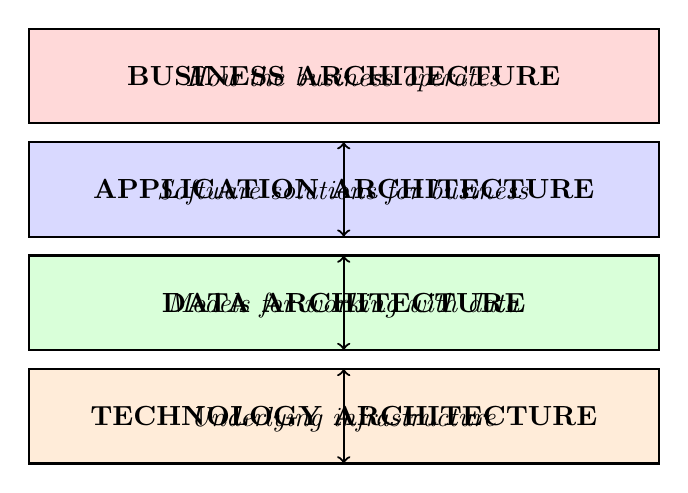
\begin{tikzpicture}[scale=0.8]
					% Business Architecture
					\draw[thick, fill=red!15] (0,0) rectangle (10,1.5) node[midway] {\textbf{BUSINESS ARCHITECTURE}};
					\node at (5,0.7) {\textit{How the business operates}};
					
					% Application Architecture
					\draw[thick, fill=blue!15] (0,-1.8) rectangle (10,-0.3) node[midway] {\textbf{APPLICATION ARCHITECTURE}};
					\node at (5,-1.1) {\textit{Software solutions for business}};
					
					% Data Architecture
					\draw[thick, fill=green!15] (0,-3.6) rectangle (10,-2.1) node[midway] {\textbf{DATA ARCHITECTURE}};
					\node at (5,-2.9) {\textit{Models for working with data}};
					
					% Technology Architecture
					\draw[thick, fill=orange!15] (0,-5.4) rectangle (10,-3.9) node[midway] {\textbf{TECHNOLOGY ARCHITECTURE}};
					\node at (5,-4.7) {\textit{Underlying infrastructure}};
					
					% Arrows showing dependency
					\draw[<->, thick] (5,-0.3) -- (5,-1.8);
					\draw[<->, thick] (5,-2.1) -- (5,-3.6);
					\draw[<->, thick] (5,-3.9) -- (5,-5.4);
				\end{tikzpicture}
			\end{center}
		\end{block}
	\end{frame}
	
	\begin{frame}{1.1 Architecture Domains Explained}
		\begin{block}{Business Architecture}
			\begin{itemize}
				\item Captures \textbf{how} a business operates
				\item Defines \textbf{business processes}
				\item Defines role of \textbf{underlying software}
				\item Ensures software doesn't become \textbf{obsolete}
			\end{itemize}
		\end{block}
		
		\begin{block}{Application Architecture}
			\begin{itemize}
				\item Defines \textbf{software solutions}
				\item Enables businesses to achieve \textbf{objectives}
				\item Adapts to \textbf{changing business requirements}
				\item Examples: CRM, ERP, HR systems
			\end{itemize}
		\end{block}
	\end{frame}
	
	\begin{frame}{1.1 Data and Technology Architecture}
		\begin{block}{Data Architecture}
			\begin{itemize}
				\item Defines \textbf{model} for working with data
				\item Manages different \textbf{sources} and \textbf{formats}
				\item Applications use data to derive \textbf{insights}
				\item Examples: Data warehouses, data lakes, ETL pipelines
			\end{itemize}
		\end{block}
		
		\begin{block}{Technology Architecture}
			\begin{itemize}
				\item Describes \textbf{underlying infrastructure}
				\item \textbf{Physical entities}: Networks, storage, hardware
				\item Shows \textbf{current state} of IT
				\item Establishes vision for \textbf{future state}
				\item Examples: Networking devices, servers, storage, software
			\end{itemize}
		\end{block}
		
		\begin{alertblock}{The Critical Trap}
			\textbf{Technology Architecture} includes \textbf{networking devices, storage, and software} - the \textbf{infrastructure} layer.
		\end{alertblock}
	\end{frame}
	
	\begin{frame}{1.1 Common EA Frameworks}
		\begin{block}{Popular Frameworks}
			\begin{tabular}{|p{3cm}|p{4cm}|p{4cm}|}
				\hline
				\textbf{Framework} & \textbf{Type} & \textbf{Best For} \\
				\hline
				TOGAF & Comprehensive & Large enterprises \\
				\hline
				Zachman & Classification & Framework integration \\
				\hline
				DODAF & Military/Government & Defense organizations \\
				\hline
				FEAF & Government & US Federal agencies \\
				\hline
				SABSA & Security-focused & Security architecture \\
				\hline
			\end{tabular}
		\end{block}
		
		\begin{exampleblock}{Key Insight}
			The goal of a risk manager is to ensure that technology architecture evolves with \textbf{minimal disruption} to IT and the business.
		\end{exampleblock}
	\end{frame}
	
	% ----------------------------------------------------------------------
	\subsection{1.2 Capability Maturity Model}
	\begin{frame}{1.2 Understanding CMM}
		\begin{block}{What is CMM?}
			\begin{itemize}
				\item \textbf{Capability Maturity Model}
				\item Developed in 1986 for US Department of Defense
				\item Assesses and improves process \textbf{maturity}
				\item Later became \textbf{CMMI} (Capability Maturity Model Integration)
			\end{itemize}
		\end{block}
		
		\begin{block}{The Five Levels}
			\begin{center}
				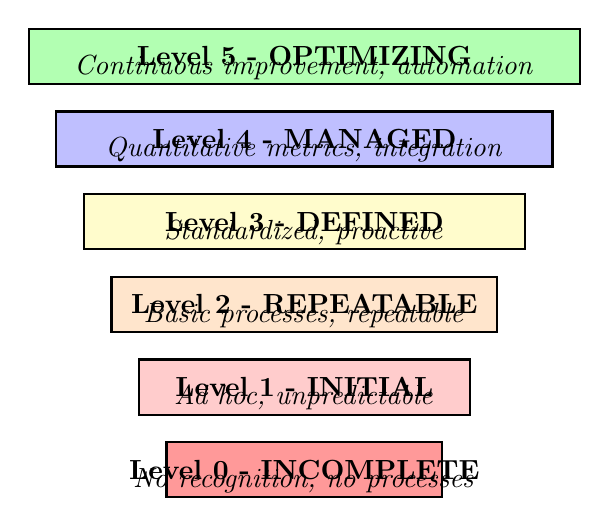
\begin{tikzpicture}[scale=0.7]
					% Level 5
					\draw[thick, fill=green!30] (0,0) rectangle (10,1) node[midway] {\textbf{Level 5 - OPTIMIZING}};
					\node at (5,0.3) {\textit{Continuous improvement, automation}};
					
					% Level 4
					\draw[thick, fill=blue!25] (0.5,-1.5) rectangle (9.5,-0.5) node[midway] {\textbf{Level 4 - MANAGED}};
					\node at (5,-1.2) {\textit{Quantitative metrics, integration}};
					
					% Level 3
					\draw[thick, fill=yellow!20] (1,-3) rectangle (9,-2) node[midway] {\textbf{Level 3 - DEFINED}};
					\node at (5,-2.7) {\textit{Standardized, proactive}};
					
					% Level 2
					\draw[thick, fill=orange!20] (1.5,-4.5) rectangle (8.5,-3.5) node[midway] {\textbf{Level 2 - REPEATABLE}};
					\node at (5,-4.2) {\textit{Basic processes, repeatable}};
					
					% Level 1
					\draw[thick, fill=red!20] (2,-6) rectangle (8,-5) node[midway] {\textbf{Level 1 - INITIAL}};
					\node at (5,-5.7) {\textit{Ad hoc, unpredictable}};
					
					% Level 0
					\draw[thick, fill=red!40] (2.5,-7.5) rectangle (7.5,-6.5) node[midway] {\textbf{Level 0 - INCOMPLETE}};
					\node at (5,-7.2) {\textit{No recognition, no processes}};
				\end{tikzpicture}
			\end{center}
		\end{block}
	\end{frame}
	
	\begin{frame}{1.2 CMM Levels Explained}
		\begin{block}{Level 0 - Incomplete}
			\begin{itemize}
				\item Enterprise does \textbf{not recognize} the need
				\item Decisions \textbf{lack credible information}
				\item No awareness of risk management
			\end{itemize}
		\end{block}
		
		\begin{block}{Level 1 - Initial}
			\begin{itemize}
				\item Risk viewed as \textbf{technical} issue
				\item \textbf{Ad hoc} skills
				\item \textbf{Episodic} risk assessments
			\end{itemize}
		\end{block}
		
		\begin{block}{Level 2 - Repeatable}
			\begin{itemize}
				\item \textbf{Basic processes} exist
				\item Risk viewed as business issue \textit{in IT}
				\item Some \textbf{repeatability}
			\end{itemize}
		\end{block}
	\end{frame}
	
	\begin{frame}{1.2 Levels 3-5}
		\begin{block}{Level 3 - Defined}
			\begin{itemize}
				\item Risk viewed as \textbf{business issue}
				\item Business knows how IT fits in \textbf{enterprise risk universe}
				\item \textbf{Workflow tools} used
				\item Processes are \textbf{standardized}
				\item \textbf{Proactive} rather than reactive
			\end{itemize}
		\end{block}
		
		\begin{block}{Level 4 - Managed}
			\begin{itemize}
				\item \textbf{Quantitative metrics} used
				\item Integrated with \textbf{ERM}
				\item Data-driven decisions
			\end{itemize}
		\end{block}
		
		\begin{block}{Level 5 - Optimizing}
			\begin{itemize}
				\item \textbf{Real-time monitoring}
				\item \textbf{Automation} of policy management
				\item \textbf{Continuous improvement}
				\item \textbf{Predictive analytics}
			\end{itemize}
		\end{block}
	\end{frame}
	
	% ============================================================
	% SECTION 2: COMPUTER NETWORKS
	% ============================================================
	\section{2. Computer Networks}
	
	% ----------------------------------------------------------------------
	\subsection{2.1 Network Models}
	\begin{frame}{2.1 TCP/IP Model}
		\begin{block}{TCP/IP Layers}
			\begin{center}
				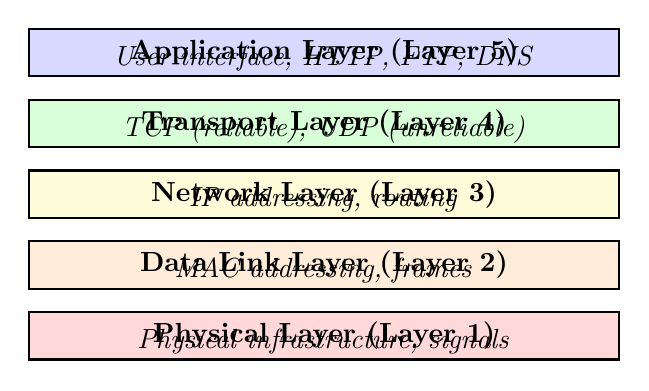
\begin{tikzpicture}[scale=0.75]
					% Layer 5
					\draw[thick, fill=blue!15] (0,0) rectangle (10,0.8) node[midway] {\textbf{Application Layer (Layer 5)}};
					\node at (5,0.3) {\textit{User interface, HTTP, FTP, DNS}};
					
					% Layer 4
					\draw[thick, fill=green!15] (0,-1.2) rectangle (10,-0.4) node[midway] {\textbf{Transport Layer (Layer 4)}};
					\node at (5,-0.9) {\textit{TCP (reliable), UDP (unreliable)}};
					
					% Layer 3
					\draw[thick, fill=yellow!15] (0,-2.4) rectangle (10,-1.6) node[midway] {\textbf{Network Layer (Layer 3)}};
					\node at (5,-2.1) {\textit{IP addressing, routing}};
					
					% Layer 2
					\draw[thick, fill=orange!15] (0,-3.6) rectangle (10,-2.8) node[midway] {\textbf{Data Link Layer (Layer 2)}};
					\node at (5,-3.3) {\textit{MAC addressing, frames}};
					
					% Layer 1
					\draw[thick, fill=red!15] (0,-4.8) rectangle (10,-4.0) node[midway] {\textbf{Physical Layer (Layer 1)}};
					\node at (5,-4.5) {\textit{Physical infrastructure, signals}};
				\end{tikzpicture}
			\end{center}
		\end{block}
		
		\begin{alertblock}{The Critical Trap}
			\textbf{Network Layer} = IP addressing (Layer 3) \\
			\textbf{Transport Layer} = TCP/UDP (Layer 4) \\
			\textbf{Application Layer} = User-facing protocols (Layer 5)
		\end{alertblock}
	\end{frame}
	
	\begin{frame}{2.1 OSI Model}
		\begin{block}{OSI Layers}
			\begin{center}
				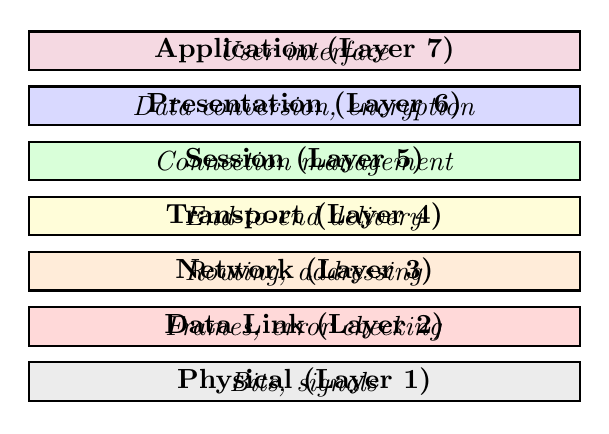
\begin{tikzpicture}[scale=0.7]
					% Layer 7
					\draw[thick, fill=purple!15] (0,0) rectangle (10,0.7) node[midway] {\textbf{Application (Layer 7)}};
					\node at (5,0.3) {\textit{User interface}};
					
					% Layer 6
					\draw[thick, fill=blue!15] (0,-1) rectangle (10,-0.3) node[midway] {\textbf{Presentation (Layer 6)}};
					\node at (5,-0.7) {\textit{Data conversion, encryption}};
					
					% Layer 5
					\draw[thick, fill=green!15] (0,-2) rectangle (10,-1.3) node[midway] {\textbf{Session (Layer 5)}};
					\node at (5,-1.7) {\textit{Connection management}};
					
					% Layer 4
					\draw[thick, fill=yellow!15] (0,-3) rectangle (10,-2.3) node[midway] {\textbf{Transport (Layer 4)}};
					\node at (5,-2.7) {\textit{End-to-end delivery}};
					
					% Layer 3
					\draw[thick, fill=orange!15] (0,-4) rectangle (10,-3.3) node[midway] {\textbf{Network (Layer 3)}};
					\node at (5,-3.7) {\textit{Routing, addressing}};
					
					% Layer 2
					\draw[thick, fill=red!15] (0,-5) rectangle (10,-4.3) node[midway] {\textbf{Data Link (Layer 2)}};
					\node at (5,-4.7) {\textit{Frames, error checking}};
					
					% Layer 1
					\draw[thick, fill=gray!15] (0,-6) rectangle (10,-5.3) node[midway] {\textbf{Physical (Layer 1)}};
					\node at (5,-5.7) {\textit{Bits, signals}};
				\end{tikzpicture}
			\end{center}
		\end{block}
	\end{frame}
	
	\begin{frame}{2.1 TCP/IP vs OSI}
		\begin{block}{Key Differences}
			\begin{tabular}{|p{2.5cm}|p{4cm}|p{4.5cm}|}
				\hline
				\textbf{Feature} & \textbf{TCP/IP} & \textbf{OSI} \\
				\hline
				Layers & 5 layers & 7 layers \\
				\hline
				Session Layer & Not separate & Separate layer (Layer 5) \\
				\hline
				Presentation Layer & Not separate & Separate layer (Layer 6) \\
				\hline
				Purpose & Practical implementation & Conceptual framework \\
				\hline
				Approach & Implemented & Theoretical \\
				\hline
			\end{tabular}
		\end{block}
		
		\begin{exampleblock}{Key Insight}
			TCP/IP is \textbf{implemented} in practice. \\
			OSI is a \textbf{conceptual} framework for understanding networks.
		\end{exampleblock}
	\end{frame}
	
	% ----------------------------------------------------------------------
	\subsection{2.2 Networking Devices}
	\begin{frame}{2.2 Networking Devices}
		\begin{block}{Device Overview}
			\begin{tabular}{|p{2.5cm}|p{4cm}|p{4.5cm}|}
				\hline
				\textbf{Device} & \textbf{OSI Layer} & \textbf{Function} \\
				\hline
				Repeater & Layer 1 (Physical) & Regenerates signal \\
				\hline
				Bridge & Layer 2 (Data Link) & Joins two networks \\
				\hline
				Switch & Layer 2 (Data Link) & Multi-port bridge, MAC addresses \\
				\hline
				Router & Layer 3 (Network) & Connects networks, IP addresses \\
				\hline
				Gateway & Layer 3+ & Connects different protocols \\
				\hline
			\end{tabular}
		\end{block}
		
		\begin{alertblock}{The Critical Trap}
			\begin{itemize}
				\item \textbf{Switch} = MAC addresses (Layer 2)
				\item \textbf{Router} = IP addresses (Layer 3)
				\item \textbf{Gateway} = Different protocols (Layer 3+)
			\end{itemize}
		\end{alertblock}
	\end{frame}
	
	% ----------------------------------------------------------------------
	\subsection{2.3 Firewalls and IDS/IPS}
	\begin{frame}{2.3 Firewall Types}
		\begin{block}{Firewall Types}
			\begin{tabular}{|p{3cm}|p{4cm}|p{4cm}|}
				\hline
				\textbf{Type} & \textbf{OSI Layer} & \textbf{Description} \\
				\hline
				Packet Filtering & Layer 3 & Compares packets to rules \\
				\hline
				Circuit-Level Gateway & Layer 5 & Monitors TCP handshakes \\
				\hline
				Application-Level Gateway & Layer 7 & Examines each layer \\
				\hline
				Stateful Inspection & Layer 3 & Tracks connections \\
				\hline
				Next-Generation & Layer 7 & Deep packet inspection \\
				\hline
			\end{tabular}
		\end{block}
		
		\begin{exampleblock}{Key Insight}
			\textbf{Application-Level Gateway} = Most secure (Layer 7) \\
			\textbf{Next-Generation} = Most advanced (Layer 7 + IPS)
		\end{exampleblock}
	\end{frame}
	
	\begin{frame}{2.3 IDS vs IPS}
		\begin{block}{Intrusion Detection Systems (IDS)}
			\begin{itemize}
				\item \textbf{Detects} potential malicious traffic
				\item \textbf{Does NOT block} traffic
				\item Sends \textbf{alerts} to security teams
				\item \textbf{Passive} system
				\item \textbf{No effect} on network throughput
			\end{itemize}
		\end{block}
		
		\begin{block}{Intrusion Prevention Systems (IPS)}
			\begin{itemize}
				\item \textbf{Detects AND blocks} malicious traffic
				\item \textbf{Active} system
				\item Implemented \textbf{in-line} with traffic
				\item May \textbf{reduce} network throughput
				\item Also called \textbf{IDS with blocking} capability
			\end{itemize}
		\end{block}
		
		\begin{alertblock}{The Critical Trap}
			\textbf{IDS} = \textit{Detects only} \\
			\textbf{IPS} = \textit{Detects AND prevents}
		\end{alertblock}
	\end{frame}
	
	% ----------------------------------------------------------------------
	\subsection{2.4 DNS and VPN}
	\begin{frame}{2.4 Domain Name System (DNS)}
		\begin{block}{What is DNS?}
			\begin{itemize}
				\item Acts as a \textbf{directory} for internet domain names
				\item Translates \textbf{domain names} to \textbf{IP addresses}
				\item Example: [www.grcmusings.com](http://www.grcmusings.com) $\to$ 162.241.252.221
				\item Critical for \textbf{user-friendliness}
				\item Application Layer protocol (Layer 7)
			\end{itemize}
		\end{block}
		
		\begin{block}{Finding IP Address}
			\begin{itemize}
				\item Use \textbf{ping} command in Command Prompt
				\item Example: \texttt{ping grcmusings.com}
				\item Shows the IP address of the domain
			\end{itemize}
		\end{block}
	\end{frame}
	
	\begin{frame}{2.4 Virtual Private Network (VPN)}
		\begin{block}{What is a VPN?}
			\begin{itemize}
				\item Creates a \textbf{secure, encrypted tunnel}
				\item Over a \textbf{less secure} network (public internet)
				\item Provides \textbf{remote access} to private networks
				\item \textbf{Encrypts} all traffic
				\item Protects data from \textbf{interception}
			\end{itemize}
		\end{block}
		
		\begin{block}{VPN Protocols}
			\begin{itemize}
				\item \textbf{IPSec} - Most secure (Network Layer)
				\item \textbf{SSL/TLS} - Transport Layer
				\item \textbf{PPTP} - Older, less secure
				\item \textbf{L2TP} - Older, less secure
			\end{itemize}
		\end{block}
		
		\begin{alertblock}{The Critical Trap}
			\textbf{IPSec} is the \textbf{MOST SECURE} VPN protocol. \\
			\textbf{PPTP} and \textbf{L2TP} are \textbf{less secure}.
		\end{alertblock}
	\end{frame}
	
	% ============================================================
	% SECTION 3: CLOUD COMPUTING
	% ============================================================
	\section{3. Cloud Computing}
	
	% ----------------------------------------------------------------------
	\subsection{3.1 Cloud Service Models}
	\begin{frame}{3.1 Cloud Service Models}
		\begin{block}{The Three Service Models}
			\begin{center}
				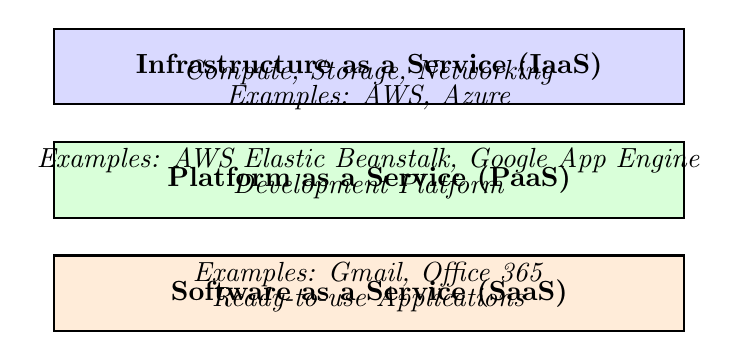
\begin{tikzpicture}[scale=0.8]
					% IaaS
					\draw[thick, fill=blue!15] (0,0) rectangle (10,1.2) node[midway] {\textbf{Infrastructure as a Service (IaaS)}};
					\node at (5,0.5) {\textit{Compute, Storage, Networking}};
					\node at (5,0.1) {\textit{Examples: AWS, Azure}};
					
					% PaaS
					\draw[thick, fill=green!15] (0,-1.8) rectangle (10,-0.6) node[midway] {\textbf{Platform as a Service (PaaS)}};
					\node at (5,-1.3) {\textit{Development Platform}};
					\node at (5,-0.9) {\textit{Examples: AWS Elastic Beanstalk, Google App Engine}};
					
					% SaaS
					\draw[thick, fill=orange!15] (0,-3.6) rectangle (10,-2.4) node[midway] {\textbf{Software as a Service (SaaS)}};
					\node at (5,-3.1) {\textit{Ready-to-use Applications}};
					\node at (5,-2.7) {\textit{Examples: Gmail, Office 365}};
				\end{tikzpicture}
			\end{center}
		\end{block}
	\end{frame}
	
%	\begin{frame}{3.1 Service Model Comparison}
%		\begin{block}{Control and Responsibility}
%			\begin{tabular}{|p{2.5cm}|p{2.5cm}|p{2.5cm}|p{2.5cm}|}
%				\hline
%				\textbf{Component} & \textbf{On-Prem} & \textbf{IaaS} & \textbf{PaaS} & \textbf{SaaS} \\
%				\hline
%				Applications & Customer & Customer & Customer & Provider \\
%				\hline
%				Data & Customer & Customer & Customer & Customer \\
%				\hline
%				Runtime & Customer & Customer & Provider & Provider \\
%				\hline
%				Middleware & Customer & Customer & Provider & Provider \\
%				\hline
%				OS & Customer & Customer & Provider & Provider \\
%				\hline
%				Virtualization & Customer & Provider & Provider & Provider \\
%				\hline
%				Servers & Customer & Provider & Provider & Provider \\
%				\hline
%				Storage & Customer & Provider & Provider & Provider \\
%				\hline
%				Networking & Customer & Provider & Provider & Provider \\
%				\hline
%			\end{tabular}
%		\end{block}
%	\end{frame}
	
	% ----------------------------------------------------------------------
	\subsection{3.2 Cloud Deployment Models}
	\begin{frame}{3.2 Cloud Deployment Models}
		\begin{block}{The Four Deployment Models}
			\begin{tabular}{|p{2.5cm}|p{4cm}|p{4.5cm}|}
				\hline
				\textbf{Model} & \textbf{Description} & \textbf{Use Case} \\
				\hline
				\textbf{Public} & Shared by general public & Broad access, SaaS \\
				\hline
				\textbf{Private} & Dedicated to one org & High security, sensitive data \\
				\hline
				\textbf{Community} & Shared by similar orgs & Research, government \\
				\hline
				\textbf{Hybrid} & Combination of models & Cloud bursting, migration \\
				\hline
			\end{tabular}
		\end{block}
		
		\begin{alertblock}{The Critical Trap}
			\begin{itemize}
				\item \textbf{Public} = Open to all
				\item \textbf{Private} = \textbf{NOT} shared with anyone
				\item \textbf{Community} = Shared with \textbf{similar} organizations
				\item \textbf{Hybrid} = Mix of public and private
			\end{itemize}
		\end{alertblock}
	\end{frame}
	
	\begin{frame}{3.2 Security Considerations}
		\begin{block}{Key Security Concerns}
			\begin{itemize}
				\item \textbf{Shared Responsibility}: Understand provider vs customer responsibilities
				\item \textbf{SLAs}: Ensure security is included
				\item \textbf{Data Breaches}: Encryption, access controls, monitoring
				\item \textbf{Compliance}: Provider must be compliant
				\item \textbf{Disaster Recovery}: Backup and recovery plans
				\item \textbf{IAM}: Strong authentication, MFA
				\item \textbf{Vendor Lock-in}: Avoid dependency on single provider
			\end{itemize}
		\end{block}
		
		\begin{exampleblock}{AWS Shared Responsibility Model}
			\begin{itemize}
				\item \textbf{AWS} responsible for: Security \textbf{of} the cloud
				\item \textbf{Customer} responsible for: Security \textbf{in} the cloud
			\end{itemize}
		\end{exampleblock}
	\end{frame}
	
	% ============================================================
	% SECTION 4: DATA LIFE CYCLE MANAGEMENT
	% ============================================================
	\section{4. Data Life Cycle Management}
	
	% ----------------------------------------------------------------------
	\subsection{4.1 Data Classification}
	\begin{frame}{4.1 Data Classification}
		\begin{block}{Why Classify Data?}
			\begin{itemize}
				\item Determines \textbf{sensitivity} of data
				\item Defines \textbf{controls} required
				\item \textbf{Directly impacts} cost of controls
				\item Enables \textbf{appropriate} protection
			\end{itemize}
		\end{block}
		
		\begin{block}{Classification Factors}
			\begin{itemize}
				\item \textbf{Regulatory requirements}: HIPAA, GDPR, PCI-DSS
				\item \textbf{Business impact}: Critical vs Public
				\item \textbf{Type}: PII, financial, health records
				\item \textbf{Access control}: Restricted vs Public
				\item \textbf{Location}: On-premises vs Cloud
			\end{itemize}
		\end{block}
		
		\begin{alertblock}{The Critical Trap}
			\textbf{Data Owner} classifies the data. \\
			\textbf{Custodian} implements the controls.
		\end{alertblock}
	\end{frame}
	
	\begin{frame}{4.1 Data Life Cycle}
		\begin{center}
			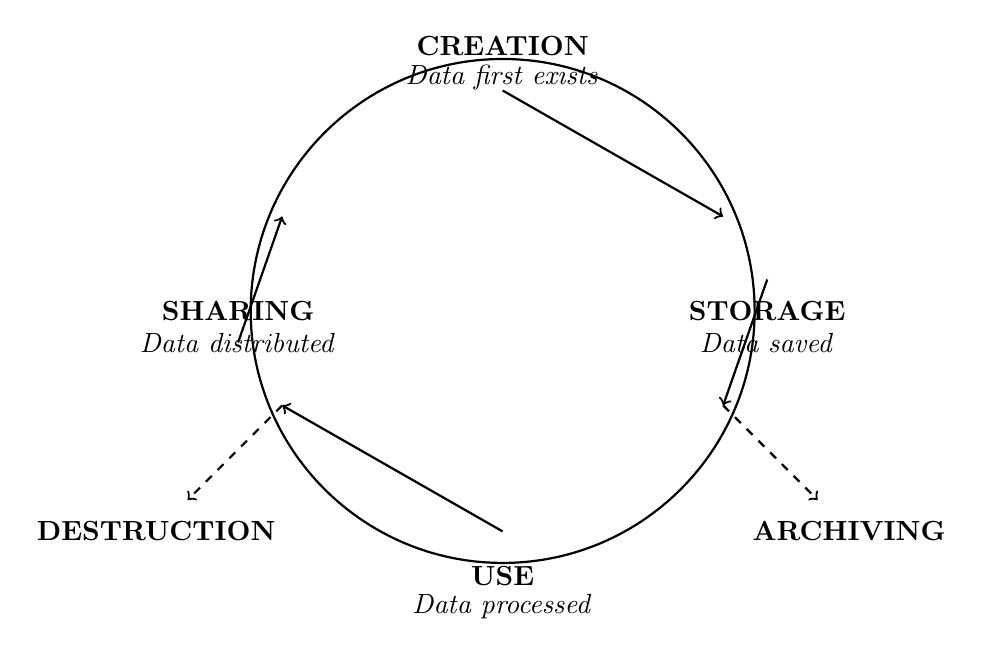
\begin{tikzpicture}[scale=0.8]
				% Cycle
				\draw[thick] (0,0) circle (4);
				
				% Creation
				\node at (0,4.2) {\textbf{CREATION}};
				\node at (0,3.7) {\textit{Data first exists}};
				
				% Storage
				\node at (4.2,0) {\textbf{STORAGE}};
				\node at (4.2,-0.5) {\textit{Data saved}};
				
				% Use
				\node at (0,-4.2) {\textbf{USE}};
				\node at (0,-4.7) {\textit{Data processed}};
				
				% Sharing
				\node at (-4.2,0) {\textbf{SHARING}};
				\node at (-4.2,-0.5) {\textit{Data distributed}};
				
				% Arrows
				\draw[->, thick] (0,3.5) -- (3.5,1.5);
				\draw[->, thick] (4.2,0.5) -- (3.5,-1.5);
				\draw[->, thick] (0,-3.5) -- (-3.5,-1.5);
				\draw[->, thick] (-4.2,-0.5) -- (-3.5,1.5);
				
				% Archiving
				\node at (5.5,-3.5) {\textbf{ARCHIVING}};
				\draw[->, thick, dashed] (3.5,-1.5) -- (5,-3);
				
				% Destruction
				\node at (-5.5,-3.5) {\textbf{DESTRUCTION}};
				\draw[->, thick, dashed] (-3.5,-1.5) -- (-5,-3);
			\end{tikzpicture}
		\end{center}
	\end{frame}
	
	\begin{frame}{4.1 Data Life Cycle Stages}
		\begin{block}{The Six Stages}
			\begin{enumerate}
				\item \textbf{Creation}: Data first comes into existence
				\item \textbf{Storage}: Data is stored and available
				\item \textbf{Use}: Data is processed for output
				\item \textbf{Sharing}: Data is shared with others
				\item \textbf{Archiving}: Data is stored for compliance
				\item \textbf{Destruction}: Data is securely destroyed
			\end{enumerate}
		\end{block}
		
		\begin{exampleblock}{Key Insight}
			More \textbf{sensitive} classification = \textbf{stronger} controls at each stage.
		\end{exampleblock}
	\end{frame}
	
	% ============================================================
	% SECTION 5: SYSTEM DEVELOPMENT LIFE CYCLE
	% ============================================================
	\section{5. System Development Life Cycle (SDLC)}
	
	% ----------------------------------------------------------------------
	\subsection{5.1 SDLC Phases}
	\begin{frame}{5.1 The SDLC Phases}
		\begin{center}
			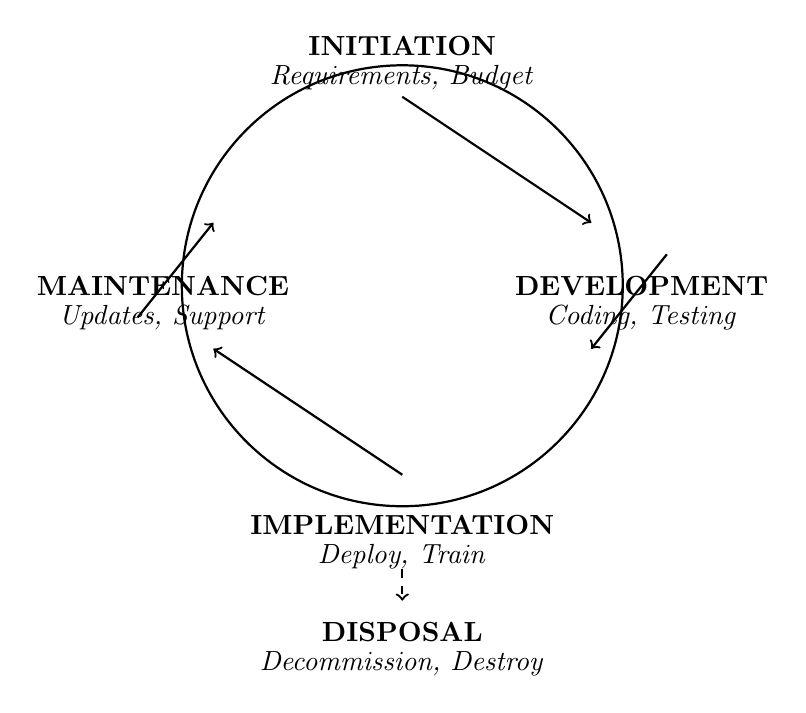
\begin{tikzpicture}[scale=0.8]
				% Phases in a circle
				\draw[thick] (0,0) circle (3.5);
				
				% Initiation
				\node at (0,3.8) {\textbf{INITIATION}};
				\node at (0,3.3) {\textit{Requirements, Budget}};
				
				% Development
				\node at (3.8,0) {\textbf{DEVELOPMENT}};
				\node at (3.8,-0.5) {\textit{Coding, Testing}};
				
				% Implementation
				\node at (0,-3.8) {\textbf{IMPLEMENTATION}};
				\node at (0,-4.3) {\textit{Deploy, Train}};
				
				% Maintenance
				\node at (-3.8,0) {\textbf{MAINTENANCE}};
				\node at (-3.8,-0.5) {\textit{Updates, Support}};
				
				% Disposal (outside)
				\node at (0,-5.5) {\textbf{DISPOSAL}};
				\node at (0,-6.0) {\textit{Decommission, Destroy}};
				
				% Arrows
				\draw[->, thick] (0,3) -- (3,1);
				\draw[->, thick] (4.2,0.5) -- (3,-1);
				\draw[->, thick] (0,-3) -- (-3,-1);
				\draw[->, thick] (-4.2,-0.5) -- (-3,1);
				\draw[->, thick, dashed] (0,-4.5) -- (0,-5);
			\end{tikzpicture}
		\end{center}
	\end{frame}
	
	\begin{frame}{5.1 Phase 1 - Initiation}
		\begin{block}{Initiation Phase}
			\begin{itemize}
				\item \textbf{First} phase of SDLC
				\item Evaluate project \textbf{feasibility}
				\item Define goals and \textbf{objectives}
				\item Identify \textbf{stakeholders}
				\item Gather \textbf{requirements}
				\item Create \textbf{project charter}
				\item \textbf{Budgeting} occurs here
			\end{itemize}
		\end{block}
		
		\begin{block}{Risks in Initiation}
			\begin{itemize}
				\item Unclear project \textbf{goals}
				\item Lack of \textbf{stakeholder support}
				\item Inadequate \textbf{budget} or \textbf{resources}
				\item Inaccurate project \textbf{requirements}
			\end{itemize}
		\end{block}
	\end{frame}
	
	\begin{frame}{5.1 Phases 2-3}
		\begin{block}{Phase 2 - Development/Acquisition}
			\begin{itemize}
				\item \textbf{Actual coding} takes place
				\item Software created based on specifications
				\item Acquire software if not building
				\item \textbf{Testing} is critical
			\end{itemize}
		\end{block}
		
		\begin{block}{Phase 3 - Implementation}
			\begin{itemize}
				\item \textbf{Install} the software system
				\item \textbf{Train} end users
				\item \textbf{Configure} and enable security
				\item Verify security \textbf{configurations}
			\end{itemize}
		\end{block}
		
		\begin{alertblock}{The Critical Trap}
			\textbf{End user training} occurs in the \textbf{IMPLEMENTATION} phase. \\
			\textbf{Budgeting} occurs in the \textbf{INITIATION} phase.
		\end{alertblock}
	\end{frame}
	
	\begin{frame}{5.1 Phases 4-5}
		\begin{block}{Phase 4 - Operation/Maintenance}
			\begin{itemize}
				\item System is \textbf{deployed}
				\item Focus: Ensure system \textbf{functions} as intended
				\item Address issues \textbf{promptly}
				\item Activities: Monitoring, bug fixes, updates, enhancements
			\end{itemize}
		\end{block}
		
		\begin{block}{Phase 5 - Disposal}
			\begin{itemize}
				\item \textbf{FINAL} stage of SDLC
				\item Remove system from \textbf{operation}
				\item \textbf{Secure destruction} of data
				\item Decommission hardware and software
				\item Ensure \textbf{no unauthorized access}
			\end{itemize}
		\end{block}
		
		\begin{alertblock}{The Critical Trap}
			\textbf{Disposal} is the \textbf{FINAL} phase of SDLC. \\
			\textbf{Initiation} is the \textbf{FIRST} phase.
		\end{alertblock}
	\end{frame}
	
	% ----------------------------------------------------------------------
	\subsection{5.2 Project Risk vs SDLC Risk}
	\begin{frame}{5.2 Project Risk vs SDLC Risk}
		\begin{block}{Project Risk}
			\begin{itemize}
				\item Risk associated with achieving \textbf{project objectives}
				\item Examples:
				\begin{itemize}
					\item Delivering on \textbf{time}
					\item Staying \textbf{within budget}
					\item Meeting \textbf{requirements}
				\end{itemize}
				\item Can be \textbf{external} (market changes) or \textbf{internal} (delays)
			\end{itemize}
		\end{block}
		
		\begin{block}{SDLC Risk}
			\begin{itemize}
				\item Risk associated with the \textbf{development process}
				\item Examples:
				\begin{itemize}
					\item \textbf{Requirements} gathering issues
					\item \textbf{Design} flaws
					\item \textbf{Coding} errors
					\item \textbf{Testing} gaps
				\end{itemize}
				\item Managed through \textbf{best practices} and \textbf{standards}
			\end{itemize}
		\end{block}
		
		\begin{alertblock}{The Critical Trap}
			\textbf{Project Risk} = Achieving project \textit{objectives} \\
			\textbf{SDLC Risk} = Development \textit{process} issues
		\end{alertblock}
	\end{frame}
	
	% ============================================================
	% SECTION 6: INFORMATION SECURITY PRINCIPLES
	% ============================================================
	\section{6. Information Security Principles}
	
	% ----------------------------------------------------------------------
	\subsection{6.1 CIA Triad}
	\begin{frame}{6.1 The CIA Triad}
		\begin{block}{Confidentiality, Integrity, Availability}
			\begin{center}
				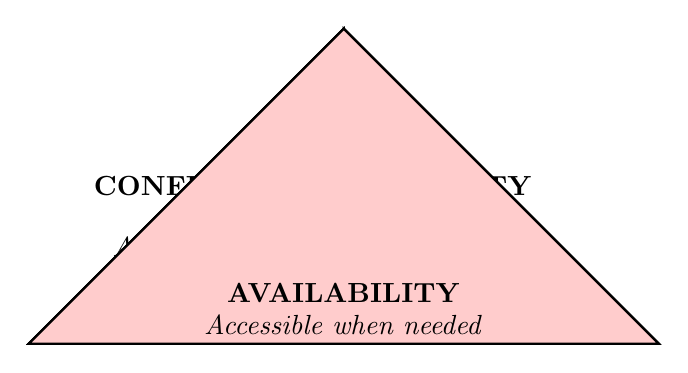
\begin{tikzpicture}[scale=0.8]
					% Triangle
					\draw[thick] (0,-3) -- (5,2) -- (10,-3) -- cycle;
					
					% Confidentiality
					\draw[thick, fill=blue!20] (0,-3) -- (5,2) -- (5,-3) -- cycle;
					\node at (3.5,-0.5) {\textbf{CONFIDENTIALITY}};
					\node at (3.5,-1.5) {\textit{Authorized access only}};
					
					% Integrity
					\draw[thick, fill=green!20] (5,2) -- (10,-3) -- (5,-3) -- cycle;
					\node at (6.5,-0.5) {\textbf{INTEGRITY}};
					\node at (6.5,-1.5) {\textit{Accurate, complete}};
					
					% Availability
					\draw[thick, fill=red!20] (0,-3) -- (10,-3) -- (5,2) -- cycle;
					\node at (5,-2.2) {\textbf{AVAILABILITY}};
					\node at (5,-2.7) {\textit{Accessible when needed}};
				\end{tikzpicture}
			\end{center}
		\end{block}
	\end{frame}
	
	\begin{frame}{6.1 CIA Definitions}
		\begin{block}{Confidentiality}
			\begin{itemize}
				\item Information accessible to \textbf{authorized users only}
				\item Protected from \textbf{unauthorized disclosure}
				\item \textbf{Need-to-know} principle
				\item \textbf{Least privilege} principle
			\end{itemize}
		\end{block}
		
		\begin{block}{Integrity}
			\begin{itemize}
				\item Information is \textbf{accurate} and \textbf{complete}
				\item Has NOT been \textbf{tampered} with
				\item Protected from \textbf{unauthorized modification}
				\item Ensures information is \textbf{trustworthy}
			\end{itemize}
		\end{block}
		
		\begin{block}{Availability}
			\begin{itemize}
				\item Information accessible to \textbf{authorized users when needed}
				\item Ensures \textbf{uninterrupted} access
				\item Protected from \textbf{downtime} and \textbf{disruptions}
			\end{itemize}
		\end{block}
	\end{frame}
	
	\begin{frame}{6.1 CIA Trade-offs}
		\begin{block}{The Three-way Trade-off}
			\begin{itemize}
				\item You \textbf{cannot} maximize all three simultaneously
				\item Trade-offs are \textbf{always} necessary
			\end{itemize}
		\end{block}
		
		\begin{block}{Confidentiality vs Availability}
			\begin{itemize}
				\item \textbf{Increasing Confidentiality}: More encryption, more authentication
				\item \textbf{Effect on Availability}: \textbf{Decreases} availability
				\item \textbf{Why}: More processing time, slower access
			\end{itemize}
		\end{block}
		
		\begin{block}{Integrity vs Availability}
			\begin{itemize}
				\item \textbf{Increasing Integrity}: More validation, more checks
				\item \textbf{Effect on Availability}: \textbf{Decreases} availability
				\item \textbf{Why}: Slows processing, delays access
			\end{itemize}
		\end{block}
	\end{frame}
	
	% ----------------------------------------------------------------------
	\subsection{6.2 Access Management}
	\begin{frame}{6.2 The IAAA Framework}
		\begin{block}{IAAA - Four Pillars of Access Management}
			\begin{tabular}{|p{2.5cm}|p{4cm}|p{4.5cm}|}
				\hline
				\textbf{Pillar} & \textbf{Description} & \textbf{Example} \\
				\hline
				\textbf{Identification} & Unique ID for each user & Username, email \\
				\hline
				\textbf{Authentication} & Prove identity & Password, biometric \\
				\hline
				\textbf{Authorization} & Define permissions & Role-based access \\
				\hline
				\textbf{Accountability} & Log and monitor & Audit trails \\
				\hline
			\end{tabular}
		\end{block}
		
		\begin{alertblock}{The Critical Trap}
			\begin{itemize}
				\item \textbf{Identification} = "Who are you?" (Username)
				\item \textbf{Authentication} = "Prove it" (Password)
				\item \textbf{Authorization} = "What can you do?" (Permissions)
				\item \textbf{Accountability} = "What did you do?" (Logging)
			\end{itemize}
		\end{alertblock}
	\end{frame}
	
	\begin{frame}{6.2 Multi-Factor Authentication}
		\begin{block}{Three Authentication Factors}
			\begin{itemize}
				\item \textbf{Something You Know}: Password, PIN, Security Questions
				\item \textbf{Something You Have}: Smart card, Token, Phone
				\item \textbf{Something You Are}: Fingerprint, Retinal scan, Voice
			\end{itemize}
		\end{block}
		
		\begin{block}{MFA Implementation}
			\begin{itemize}
				\item Uses \textbf{two or more} factors
				\item Example: Password + Fingerprint
				\item Much \textbf{more secure} than single factor
				\item \textbf{Recommended} for all systems
			\end{itemize}
		\end{block}
		
		\begin{exampleblock}{Key Insight}
			Username + Password = \textbf{Single Factor} (Not MFA) \\
			Password + Fingerprint = \textbf{Multi-Factor}
		\end{exampleblock}
	\end{frame}
	
	\begin{frame}{6.2 Segregation of Duties (SOD)}
		\begin{block}{What is SOD?}
			\begin{itemize}
				\item \textbf{Prevents} internal fraud
				\item No single individual has \textbf{complete control}
				\item \textbf{Distributes} access across multiple people
				\item \textbf{Prevents} conflicts of interest
				\item \textbf{Required} for SOX and PCI DSS compliance
			\end{itemize}
		\end{block}
		
		\begin{block}{SOD Example}
			\begin{itemize}
				\item Person \textbf{A} approves invoices
				\item Person \textbf{B} processes payments
				\item Person \textbf{C} reconciles accounts
				\item \textbf{No single person} can commit fraud alone
			\end{itemize}
		\end{block}
		
		\begin{alertblock}{The Critical Trap}
			\textbf{SOD} = \textit{Separation of Duties} \\
			\textbf{Not} the same as separation of \textit{roles} or \textit{functions}.
		\end{alertblock}
	\end{frame}
	
	% ----------------------------------------------------------------------
	\subsection{6.3 Encryption and Hashing}
	\begin{frame}{6.3 Symmetric vs Asymmetric Encryption}
		\begin{block}{Symmetric Encryption}
			\begin{itemize}
				\item \textbf{Single key} for encryption and decryption
				\item \textbf{Faster} and more efficient
				\item \textbf{Drawback}: Key must be securely shared
				\item Example: \textbf{AES}, DES
			\end{itemize}
		\end{block}
		
		\begin{block}{Asymmetric Encryption}
			\begin{itemize}
				\item \textbf{Two keys}: Public key + Private key
				\item \textbf{Slower} but more secure
				\item \textbf{Advantage}: Secure key exchange
				\item Example: \textbf{RSA}, ECC
			\end{itemize}
		\end{block}
		
		\begin{alertblock}{The Critical Trap}
			\textbf{Symmetric} = Same key (faster, less secure) \\
			\textbf{Asymmetric} = Different keys (slower, more secure)
		\end{alertblock}
	\end{frame}
	
	\begin{frame}{6.3 Hashing}
		\begin{block}{What is Hashing?}
			\begin{itemize}
				\item Converts arbitrary input to \textbf{fixed-size output}
				\item \textbf{One-way} function (cannot reverse)
				\item \textbf{Unique} output for each input
				\item \textbf{Minor changes} = completely different hash
				\item Provides \textbf{integrity} verification
			\end{itemize}
		\end{block}
		
		\begin{block}{Hashing Uses}
			\begin{itemize}
				\item \textbf{Password storage} (never store plaintext)
				\item \textbf{Data integrity} checks
				\item \textbf{Digital signatures}
				\item \textbf{Fingerprints} for files
			\end{itemize}
		\end{block}
		
		\begin{exampleblock}{Key Insight}
			Hashing is \textbf{NOT} reversible. \\
			Encryption IS reversible (with the key).
		\end{exampleblock}
	\end{frame}
	
	% ----------------------------------------------------------------------
	\subsection{6.4 Digital Signatures}
	\begin{frame}{6.4 Digital Signatures}
		\begin{block}{What is a Digital Signature?}
			\begin{itemize}
				\item Provides \textbf{authenticity}, \textbf{integrity}, and \textbf{non-repudiation}
				\item \textbf{DOES NOT} provide confidentiality on its own
				\item Uses \textbf{hashing} + \textbf{asymmetric encryption}
			\end{itemize}
		\end{block}
		
		\begin{block}{What Digital Signatures Provide}
			\begin{tabular}{|p{3cm}|p{4cm}|p{4cm}|}
				\hline
				\textbf{Feature} & \textbf{Provided?} & \textbf{Why} \\
				\hline
				Integrity & Yes & Hash ensures no tampering \\
				\hline
				Authenticity & Yes & Private key proves identity \\
				\hline
				Non-repudiation & Yes & Sender cannot deny \\
				\hline
				Confidentiality & \textbf{NO} & Message remains unencrypted \\
				\hline
			\end{tabular}
		\end{block}
		
		\begin{alertblock}{The Critical Trap}
			Digital signatures provide \textbf{Integrity + Non-repudiation}. \\
			They do \textbf{NOT} provide \textbf{Confidentiality}.
		\end{alertblock}
	\end{frame}
	
	\begin{frame}{6.4 Signed vs Encrypted}
		\begin{block}{Options for Message Security}
			\begin{tabular}{|p{3cm}|p{4cm}|p{4cm}|}
				\hline
				\textbf{Method} & \textbf{Provides} & \textbf{Not Provides} \\
				\hline
				Signed Only & Integrity, Non-repudiation & Confidentiality \\
				\hline
				Encrypted Only & Confidentiality & Integrity, Non-repudiation \\
				\hline
				Signed + Encrypted & \textbf{ALL THREE} & Nothing \\
				\hline
			\end{tabular}
		\end{block}
		
		\begin{exampleblock}{Key Insight}
			To get \textbf{ALL THREE} (Confidentiality, Integrity, Non-repudiation): \\
			\textbf{Signed AND Encrypted}
		\end{exampleblock}
	\end{frame}
	
	% ----------------------------------------------------------------------
	\subsection{6.5 Public Key Infrastructure}
	\begin{frame}{6.5 Understanding PKI}
		\begin{block}{What is PKI?}
			\begin{itemize}
				\item \textbf{Public Key Infrastructure}
				\item Establishes, manages, distributes, and revokes \textbf{digital certificates}
				\item Uses \textbf{public key cryptography}
				\item Relies on \textbf{trusted third parties} (CAs)
			\end{itemize}
		\end{block}
		
		\begin{block}{PKI Components}
			\begin{itemize}
				\item \textbf{CA} (Certificate Authority) - Issues certificates
				\item \textbf{Certificate} - Links public key to identity
				\item \textbf{CRL} (Certificate Revocation List) - Revoked certificates
				\item \textbf{Registration Authority} - Verifies identities
			\end{itemize}
		\end{block}
	\end{frame}
	
	\begin{frame}{6.5 PKI Single Point of Failure}
		\begin{block}{The SPOF Risk}
			\begin{itemize}
				\item The \textbf{CA} holds the private key
				\item If CA's private key is \textbf{compromised}:
				\begin{itemize}
					\item All certificates become \textbf{untrustworthy}
					\item Massive \textbf{security} breach
					\item \textbf{Widespread} impact
				\end{itemize}
				\item This is a \textbf{single point of failure}
			\end{itemize}
		\end{block}
		
		\begin{alertblock}{The Critical Trap}
			\textbf{CA} is the \textbf{SPOF} in PKI. \\
			\textbf{Certificates} are NOT the SPOF.
		\end{alertblock}
	\end{frame}
	
	% ============================================================
	% SECTION 7: COMMON EXAM TRAPS
	% ============================================================
	\section{7. Common Exam Traps}
	
	% ----------------------------------------------------------------------
	\subsection{7.1 IT and Security Traps}
	\begin{frame}{7.1 Common Exam Traps - IT and Security}
		\begin{block}{Trap \#1: Network Layers}
			\begin{itemize}
				\item \textbf{Common Mistake}: Confusing TCP/IP and OSI layers
				\item \textbf{Correct}:
				\begin{itemize}
					\item TCP/IP: 5 layers (Application, Transport, Network, Data Link, Physical)
					\item OSI: 7 layers (Application, Presentation, Session, Transport, Network, Data Link, Physical)
				\end{itemize}
			\end{itemize}
		\end{block}
		
		\begin{block}{Trap \#2: Cloud Models}
			\begin{itemize}
				\item \textbf{Common Mistake}: Confusing deployment models
				\item \textbf{Correct}:
				\begin{itemize}
					\item Public = Shared
					\item Private = Dedicated
					\item Community = Shared with similar orgs
					\item Hybrid = Mix
				\end{itemize}
			\end{itemize}
		\end{block}
	\end{frame}
	
	\begin{frame}{7.1 More Common Traps}
		\begin{block}{Trap \#3: Encryption Types}
			\begin{itemize}
				\item \textbf{Common Mistake}: Thinking symmetric is more secure
				\item \textbf{Correct}: \textbf{Asymmetric} is more secure (but slower)
				\item \textbf{Symmetric}: Faster, single key
				\item \textbf{Asymmetric}: Slower, key pair
			\end{itemize}
		\end{block}
		
		\begin{block}{Trap \#4: Digital Signatures}
			\begin{itemize}
				\item \textbf{Common Mistake}: Thinking digital signatures provide confidentiality
				\item \textbf{Correct}: Digital signatures provide \textbf{integrity and non-repudiation} only
				\item \textbf{Confidentiality} requires \textbf{encryption}
			\end{itemize}
		\end{block}
	\end{frame}
	
	% ============================================================
	% SECTION 8: QUICK REFERENCE
	% ============================================================
	\section{8. Quick Reference}
	
	% ----------------------------------------------------------------------
	\subsection{8.1 IT and Security Reference}
	\begin{frame}{8.1 Quick Reference - IT Architecture}
		\begin{block}{Network Layers Summary}
			\begin{tabular}{|p{2.5cm}|p{4cm}|p{4.5cm}|}
				\hline
				\textbf{Layer} & \textbf{Function} & \textbf{Examples} \\
				\hline
				Physical (L1) & Bits, signals & Cables, hubs \\
				\hline
				Data Link (L2) & Frames, MAC & Switches, bridges \\
				\hline
				Network (L3) & Packets, IP & Routers, firewalls \\
				\hline
				Transport (L4) & TCP/UDP & Load balancers \\
				\hline
				Session (L5) & Connections & Session management \\
				\hline
				Presentation (L6) & Encryption & SSL/TLS \\
				\hline
				Application (L7) & User interface & HTTP, DNS, FTP \\
				\hline
			\end{tabular}
		\end{block}
	\end{frame}
	
	\begin{frame}{8.1 Quick Reference - Cloud}
		\begin{block}{Cloud Service Models}
			\begin{tabular}{|p{2.5cm}|p{4cm}|p{4.5cm}|}
				\hline
				\textbf{Model} & \textbf{Description} & \textbf{Examples} \\
				\hline
				IaaS & Infrastructure (Compute, Storage, Network) & AWS, Azure \\
				\hline
				PaaS & Development Platform & Elastic Beanstalk, App Engine \\
				\hline
				SaaS & Ready-to-use Applications & Gmail, Office 365 \\
				\hline
			\end{tabular}
		\end{block}
		
		\begin{block}{Cloud Deployment Models}
			\begin{tabular}{|p{2.5cm}|p{4cm}|p{4.5cm}|}
				\hline
				\textbf{Model} & \textbf{Description} & \textbf{Use Case} \\
				\hline
				Public & Shared by all & Broad access \\
				\hline
				Private & Dedicated & High security \\
				\hline
				Community & Shared by similar orgs & Research \\
				\hline
				Hybrid & Mix & Migration \\
				\hline
			\end{tabular}
		\end{block}
	\end{frame}
	
	\begin{frame}{8.1 Quick Reference - Security}
		\begin{block}{Access Management}
			\begin{tabular}{|p{2.5cm}|p{4cm}|p{4.5cm}|}
				\hline
				\textbf{Concept} & \textbf{Question} & \textbf{Example} \\
				\hline
				Identification & "Who are you?" & Username \\
				\hline
				Authentication & "Prove it" & Password, MFA \\
				\hline
				Authorization & "What can you do?" & Permissions \\
				\hline
				Accountability & "What did you do?" & Logs, Audit \\
				\hline
			\end{tabular}
		\end{block}
		
		\begin{block}{Cryptography Summary}
			\begin{tabular}{|p{2.5cm}|p{4cm}|p{4.5cm}|}
				\hline
				\textbf{Concept} & \textbf{Description} & \textbf{Use} \\
				\hline
				Symmetric & One key & Fast encryption \\
				\hline
				Asymmetric & Key pair & Secure exchange \\
				\hline
				Hashing & One-way & Integrity \\
				\hline
				Digital Signature & Hash + Asymmetric & Authentication \\
				\hline
			\end{tabular}
		\end{block}
	\end{frame}
	
	\begin{frame}{Final Advice - Section 4}
		\begin{block}{Information Technology and Security}
			\centering
			\vspace{0.3cm}
			\textbf{Remember:}
			\begin{itemize}
				\item \textbf{Routers} = IP (Layer 3); \textbf{Switches} = MAC (Layer 2)
				\item \textbf{IDS} = Detects; \textbf{IPS} = Detects AND Prevents
				\item \textbf{IPSec} = Most secure VPN protocol
				\item \textbf{Public} = Shared; \textbf{Private} = Dedicated; \textbf{Community} = Similar orgs
				\item \textbf{Symmetric} = Single key; \textbf{Asymmetric} = Key pair
				\item \textbf{Digital Signatures} = Integrity + Non-repudiation (NOT confidentiality)
				\item \textbf{CA} = SPOF in PKI
			\end{itemize}
			\vspace{0.5cm}
			\textbf{Good Luck on Your CRISC Exam!}
		\end{block}
	\end{frame}
	
	% ============================================================
	% END OF PRESENTATION
	% ============================================================
	
\end{document}